\chapter{Implementation}
\section{Hardware}
\begin{wrapfigure}{r}{0.24\textwidth}
    \includegraphics[width=0.9\linewidth]{YHDC-SCT013.jpg}
    \caption{\protect\raggedright YHDC-SCT013}
    %\vspace{-30pt}
    \label{fig:yhdc}
\end{wrapfigure}
As discussed in the introduction, there are multiple ways to collect data. For this project, we wanted a cheap solution easily usable for anyone wanting to use the project; making it more affordable for both users and contributors. This is why we use a generic split-core current transformer, like the one on \autoref{fig:yhdc}. It works using the magnetic field around the wire we monitor to produce a proportional (in this case smaller) current as the one it is clamped around. It is simply wired into the sound card of any computer. This allows getting a sampling of more than 40kHz on most sound cards. However, we are going to sample at only around  4kHz since it seems to be as efficient for our current algorithm.

During the development of the project a laptop was used but since the \acrshort{cpu} usage is very low, a single board computer running Linux (like a Raspberry Pi) should be more than enough to do the job, provided that it has an input on which you can plug the split core current transformer. Note that the split core current transformer can also be plugged into an external USB sound card for instance.


\section{Architecture}
\begin{figure}
    \centering
    \includegraphics[width=\textwidth]{img/diagram.png}
    \caption{Class Diagram}
    \label{fig:class_diagram}
\end{figure}
The project is made to be modular. It is divided into multiple modules aiming at one particular task at a time. The identified tasks are as follow: gather the data, detect when there is a change in the data (i.e. the state of an appliance has changed) and finally detect what appliance it is that has changed. The process is described on \autoref{fig:process_diagram}. Everything is made so that the disaggregation can be made with different types of input data. In this case, we only use a current meter, but the only thing we need to redefine if we change the input data (like adding readings from a voltmeter or/and using the V-I trajectory -- see \autoref{section-vi}) would be to change the distance between two data points.

\tikzset{
    mynode/.style={rectangle,rounded corners,draw=black,very thick, inner sep=0.5em, minimum size=3em, text centered},
    method/.style={ellipse,draw=black,very thick, inner sep=0.01em, minimum size=3em, text centered},
    myarrow/.style={-triangle 45, >=latex', shorten >=1pt, very thick},
    mylabel/.style={text width=7em, text centered} 
} 

\begin{figure}
    \centering
    \begin{tikzpicture}[node distance=2cm, auto]  
    \node[mynode, fill=blue!30] (new_data) {New data};
    \node[mynode, left=1cm of new_data,draw=white] (start) {Start};
    \node[mynode, above right=1cm of new_data] (smoothen_base) {Smoothen Base};
    \node[mynode, below right=1cm of new_data] (smoothen_signal) {Smoothen Signal};
    \node[mynode, below left=of smoothen_signal] (add_data) {Add data to appliance};
    \node[mynode, below right=of smoothen_signal] (new_appliance) {Create new appliance};
    \node[mynode, below = 3cm of smoothen_signal] (signal) {Signal AND New base};
    \node[method, below = 0.5cm of smoothen_signal] (closest) {Get closest};
    \node[method, right = 0.5cm of new_data] (detect) {Detect ?};
    
    \draw[myarrow] (new_data) -- node [text width=2.5cm,below,align=center,sloped] {no} (smoothen_base);
    \draw[myarrow] (new_data) -- node [text width=2.5cm,above,align=center,sloped] {yes} (smoothen_signal);
    \draw[myarrow] (smoothen_signal) -- node [text width=2.5cm,below,align=center,sloped] {Distance below threshold} (add_data);
    \draw[myarrow] (smoothen_signal) -- node [text width=2.5cm,below,align=center,sloped] {Distance above threshold} (new_appliance);
    \draw[myarrow] (add_data) -- (signal);
    \draw[myarrow] (new_appliance) -- (signal);
    \draw[myarrow,dashed] (smoothen_signal) to [out=0,in=50,loop,looseness=4] node [text width=2.5cm,above,align=center,sloped]{Repeat}(smoothen_signal);
    \draw[myarrow] (signal.west) -- ++(-5.6,0) -- ++(0,4) -| (new_data);
    \draw[myarrow] (smoothen_signal.east) -- ++(1.5,0) -- ++(0,5) -| (new_data);
    \draw[myarrow] (smoothen_base.west) -- ++(-1,0) -| (new_data);
    \draw[myarrow] (start) -- (new_data);
    \end{tikzpicture}
    \caption{Process Diagram}
    \label{fig:process_diagram}
\end{figure}


{\color{red}define signal} %TODO

In order to detect when changes in the signal occur, we need to have a base signal. This base signal is the one we should continuously have while there is no change in the network. Because there is a lot of noise due to small variations in the \acrshort{emi} -- due to changes in power needs of the appliances -- , readings errors, and changes in the frequency of the electricity provider -- due to the imbalance of the production and the consumption --, we continuously need to smooth the base signal. This smoothing occurs only if the read signal is not too far from the base signal, which is decided by \texttt{EventDetector}. If it is too far, then the few next readings are taken together and the mean is computed. The difference between this mean and the base signal is expected to be the signal emitted by the new appliance. If that appliance has already been registered, the difference with the mean computed and the base signal should be close to the signal and a copy of the data will automatically be added in the record of the appliance; if not a new appliance will be registered containing the new signal.

To illustrate this, \autoref{fig:state-before} and \autoref{fig:state-after} show the state of the decision algorithm right before and after an event was detected on a dummy example. The red line represents the base signal, that is the agglomeration of all the signals emitted by the appliances emitting \acrshort{emi} at that particular moment. An appliance just changed state, so the current measured signal, which is drawn in blue, has changed. If the difference is big enough, we wait a few moments to try to get rid of the noise in the signal and smooth the difference with the base. That smoothed difference is compared to existing appliances to try to detect which appliance is the cause for changing the signal. The base signal also changes and we get in the state represented on \autoref{fig:state-after}, where the difference between the current signal and the base signal should only be noise.

\begin{figure}
\begin{subfigure}[t]{0.49\textwidth}
    \centering
    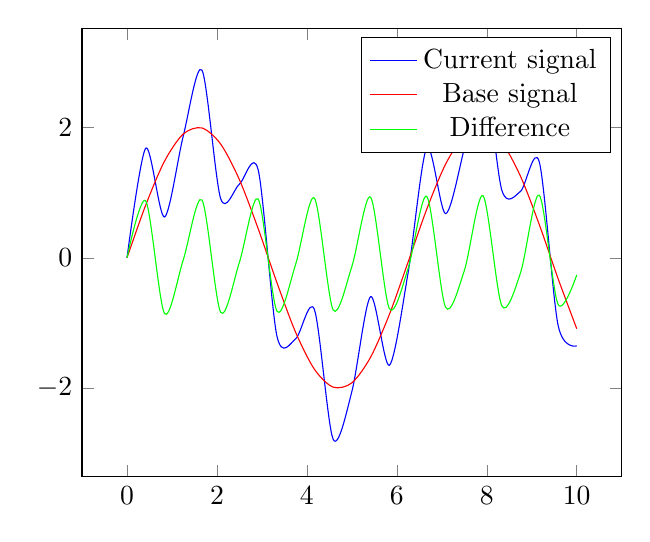
\begin{tikzpicture}[scale=1]
        \begin{axis}[domain=0:10]
            \addplot[mark=none,blue,smooth] {2*sin(deg(x))+sin(deg(5*x))}; 
            \addplot[mark=none,red,smooth] {2*sin(deg(x))};
            \addplot[mark=none,green,smooth] {sin(5*deg(x))};
            \legend{Current signal,Base signal,Difference}
        \end{axis}
    \end{tikzpicture}
    \caption{State right before an event is detected\\}
    \label{fig:state-before}
\end{subfigure}
\begin{subfigure}[t]{0.49\textwidth}
    \centering
    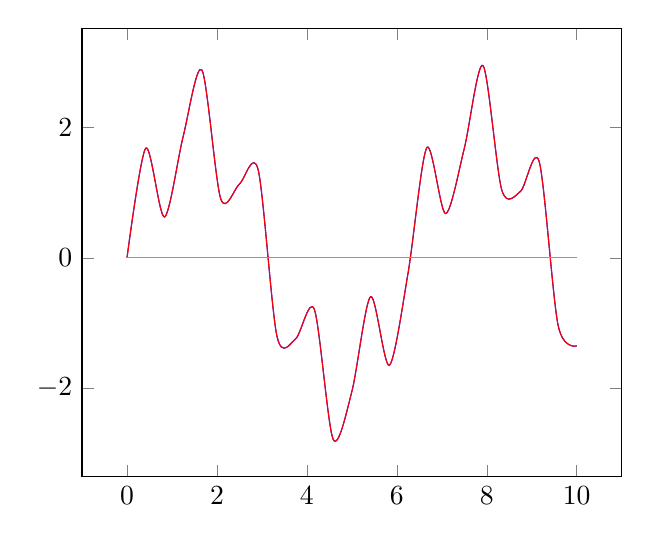
\begin{tikzpicture}[scale=1]
        \begin{axis}[domain=0:10,legend pos=outer north east]
            \addplot[mark=none,blue,smooth] {2*sin(deg(x))+sin(deg(5*x))}; 
            \addplot[mark=none,red,smooth] {2*sin(deg(x))+sin(deg(5*x))};
            \addplot[mark=none,green,smooth] {0};
            %\legend{Current signal,Base signal,Difference}
        \end{axis}
    \end{tikzpicture}
    \caption{State right after an event is detected,\\ and until something else happens on the \\network}
    \label{fig:state-after}
\end{subfigure}
\caption{Change in state}
\label{fig:change-state}
\end{figure}





\section{Algorithms chosen}
\subsection{Fast Fourier Transform}
The raw data we are measuring is actually a waveform. There are some things we can compare between two waveforms, like its maximum values at a certain point, but what we want is the amplitude of every individual frequency outputted by the sum of all appliances. This is done with a \acrshort{ft}.

There are many different types of Fourier Transforms. Because we are sampling the signal, we have to use some kind of \acrshort{dft}. The one chosen is the \acrshort{rfft} because it is optimized to be faster when the input signal is only real.

For reasons enunciated in \autoref{section:nyquist}, we will only look at the real part of the \acrshort{rfft}, as we do not want the results to change because of the difference of phase between the sampling and the input signal.

\subsection{Filtering}
There can be a lot of noise when we measure the current. This has been discussed in \autoref{section-smps}. Also, as we have discussed in \autoref{section:nyquist}, the phase shifting for the sampling may be a problem in some cases.

The combination of those two factors makes the \acrshort{fft} hard to use for comparison between two sets of sampling like we would like to do. In order to illustrate this, \autoref{fig:unfiltered_signal} shows two signals with noise. The first one is the same as the second one but the sampling started 5ms later. 

When we try to filter out the noise by just setting to 0 the values that are below 2 times the mean of \acrshort{fft} values (in this case), we see that the result is not the same depending on the time at which we started sampling. Even though the results of the \acrshort{ft} are indeed different, the sum of absolute value of the differences between the two right graphs is smaller than the one of the two middle graphs.
\begin{figure}
    \centering
    \includegraphics[width=\textwidth]{img/unfiltered.png}
    \caption{Trying to filter out noise}
    \label{fig:unfiltered_signal}
\end{figure}
\begin{figure}
    \centering
    \includegraphics[trim={0 0 0 0.1cm},clip,height=0.99\textwidth, angle =90]{img/filter.png}
    \caption{Filtering out noise with smoothing}
    \label{fig:smooth_signal}
\end{figure}

\subsection{KNN}\label{section:knn}
The \acrshort{knn} algorithm was chosen because it doesn't require training strictly speaking. The training actually is just the gathering of data. This allows seeing quickly how the detecting behaves when the number of data points is growing. However, once the number of training points is bigger, we could easily take another decision technique like a \acrshort{svm}, which is doing much better when the number of training points is huge, and the number of dimensions is big.

There was no need in this case because we were limited by the size of our training set, but \acrshort{knn} also requires to use prototype methods when the number of samples gets bigger. This could be done in a separate thread but needs to be taken into consideration.

Also, in this case, a value of 5 for $k$ was chosen because of the lack of data. But some cross-validation for choosing the value might improve the efficiency of the algorithm.

A problem with this way of using k-NN is however that if there are imprecision's during the sampling of the signal, the \acrshort{dft} could put part of the value of $X[i]$ in $X[i+1]$. For instance, reading a signal of 5kHz as a signal of 5.2kHz. This would lead to a very bad performance of the k-NN.
However, like in \cite{gupta2010electrisense}, we could approximate the \acrshort{dft} by multiple Gaussian curves and use \acrshort{knn} with the parameters of the Gaussian curves.

Another thing worth mentioning is that when I tried to normalize the data around the mean with a variance of 1, the results became really bad. This is because when we normalized the data, we give as much importance to the frequencies that consist mostly of noise than to frequencies that consist mostly of interesting frequencies, as the distance metric we use is simply the euclidian distance between the vector produced by the \acrshort{rfft}.


\subsection{Change in vectors}
In order to detect when there is a change in the \acrshort{dft} values, I used an algorithm inspired by the TCP slow start.

We start by comparing the length (the euclidian norm was chosen) between the base \acrshort{dft} vector and the current reading's \acrshort{dft} vector. If it is below a threshold, we reduce that threshold linearly and repeat that forever. When a reading produces a \acrshort{dft} which difference with a base is greater than the threshold, we augment the threshold exponentially and increment a counter. If the counter gets above a certain value, an event is detected. The counter is decremented every time the difference between the \acrshort{dft} is not greater than the threshold.

The minimum threshold should be close to 0, and the maximum threshold should be big enough to never be a trigger on its own. This way, every event should be detectable. This method ensures that small changes are still detected even if the signal is already strong.

The advantages of this method comparing to the method used by \cite{bruneel2018energy} (the T-Test, see \autoref{section:low-freq}) is that is is much less computationally intensive. However, it needs a tuning of parameters which is less robust than the T-Test, for choosing the rate at which the threshold increases and decreases, as well as choosing how much times the threshold can be exceeded.

In practice, very few false events are detected, and a vast majority of true events are detected. The exception to this is when there are high power appliances that have too much variation over the time. This causes the threshold to be a little too far to detect small appliances.
